\chapter{Methodology}

\section{Datasets and models}

% \begin{itemize}
%     \item MNIST, FashionMNIST and (maybe?) show the synthetic datasets
%     \item Describe the model(s) used
% \end{itemize}

For evaulation we have used the MNIST~\cite{deng2012mnist} and FashionMNIST~\cite{xiao2017fashionmnistnovelimagedataset} datasets
with the predefined training and testing splits.
We have also used synthetic 2D and 3D binary classification datasets for more easily interpretable experiments.
They are shown in Figures~\ref{fig:synthetic-datasets-2d} and \ref{fig:synthetic-datasets-3d}.
with each dataset consisting of $10000$ points, uniformly sampled from $[ - 1, 1]^2$
and split into training and testing sets with a ratio of $0.8:0.2$.

\todo{Maybe drop 3D}

\todo{Describe model for 2D/3D if we need that}

For MNIST and FashionMNIST, we have used:
\begin{enumerate}
    \item A simple feed-forward neural network with layer sizes
    $784, 512, 128, 16, 10$, ReLU activations and a softmax output layer.
    % This network is later denoted as ``FC''.
    \item A convolutional neural network with a modification of the architecture given in
    \href{https://github.com/pytorch/examples/tree/main/mnist}{https://github.com/pytorch/examples/tree/main/mnist}.
    The modifications are:
    \begin{enumerate}
        \item Addition of the \verb|scale| parameter, which allows us to change the neural network width.
        It is a multiplicative factor for the number of channels in the convolutional layers and number of neurons in the fully connected layers.
        \item Addition of the \verb|extra_cnn| parameter, which adds convolutional layers with $64 \cdot \verb|scale|$ channels, $3 \times 3$ kernel size,
        1 pixel padding and stride, as well as a ReLU activation.
        \item Additon of the \verb|extra_linear| parameter, which similarly adds a fully connected layer with $128 \cdot \verb|scale|$ neurons,
        as well as a ReLU activation.
    \end{enumerate}
\end{enumerate}

\begin{figure}
    \centering
    % \begin{subfigure}{0.45\textwidth}
    %     \resizebox{\textwidth}{!}{
    %         \begin{tikzpicture}
    %             \begin{axis}[
    %                 enlargelimits=false,
    %             ]
    %             \addplot+[
    %                 only marks,
    %                 scatter,
    %                 mark size=2pt,
    %                 scatter src=explicit]
    %             table[meta=class]
    %             {data/2d/manyholes.dat};
    %             \end{axis}
    %         \end{tikzpicture}
    %     }
    %     \caption{Many holes dataset}
    % \end{subfigure}
    % \begin{subfigure}{0.45\textwidth}
    %     \resizebox{\textwidth}{!}{
    %         \begin{tikzpicture}
    %             \begin{axis}[
    %                 enlargelimits=false,
    %             ]
    %             \addplot+[
    %                 only marks,
    %                 scatter,
    %                 mark size=2pt,
    %                 scatter src=explicit]
    %             table[meta=class]
    %             {data/2d/nested.dat};
    %             \end{axis}
    %         \end{tikzpicture}
    %     }
    %     \caption{Nested annuli dataset}
    % \end{subfigure}
    \caption{Synthetic 2D datasets}
    \label{fig:synthetic-datasets-2d}
\end{figure}

\section{Metrics and evaluation}

% \begin{itemize}
%     \item Wasserstein distance
%     \item Total bar length
% \end{itemize}

\todo{Explain how and why we use those}

\begin{definition}
    For \(q \geq 1\), the \emph{Wasserstein distance} between two persistence diagrams
    $\dgm_p(\mathcal{F})$ and $\dgm_p(\mathcal{G})$ is defined as
    \begin{equation}
        d_{W, q}(\dgm_p(\mathcal{F}), \dgm_p(\mathcal{G}))
        = \left[\inf_{\pi \in \Pi} \left(\sum_{x \in \dgm_p(\mathcal{F})}
        \norm{x - \pi(x)}_{\infty}^q\right)\right]^{1 / q}
    \end{equation}
\end{definition}

\begin{definition}
    The \emph{total bar length} of a persistence diagram $\dgm_p(\mathcal{F})$ is defined as
    \begin{equation}
        \sum_{(b, d) \in \dgm_p(\mathcal{F})} d - b
    \end{equation}
\end{definition}

\section{Simplicial complex}

% \begin{itemize}
    % \item Labeled Vietoris-Rips complex
    % \item Usage of \texttt{ripser++} and \texttt{giotto-ph}
    % \item Generalization to multiclass classification
%     \item Circumcircle filtering (show why it's needed in 2D, but not in high-dim)
%     \item Dowker complex
% \end{itemize}

We use the Labeled Vietoris-Rips complex, as presented in~\cite{ramamurthy2018topologicaldataanalysisdecision}.
To improve computational performance, we used the \verb|ripser++|~\cite{zhang2020gpu}
and the \verb|giotto-ph|~\cite{burella2021giottoph} packages for the Vietoris-Rips persistence barcode computation.
Both of these methods have shown lower runtime than the original
\verb|ripser|~\cite{Bauer2021Ripser} package.
However, due to GPU memory limitations, we use \verb|giotto-ph| in all experiments.

In previous research~\cite{ramamurthy2018topologicaldataanalysisdecision,li2020finding}\todo{maybe more},
classification datasets with \(n > 2\) classes were split into
\(\binom{n}{2}\) binary classification problems.
This process loses topological information, as shown in an example dataset
in Figure~\ref{fig:binarization}.
The decision boundary for all three clsases (\ref{fig:binarization:all})
has a non-trivial first homology group \(H_1\).
This is not the case for any binary classification problem for this dataset
(\ref{fig:binarization:rg}, \ref{fig:binarization:gb}).
Moreover, the decision boundary is disconnected for the red and green subdataset,
but connected for the full dataset.

\begin{figure}
    \centering
    \begin{subfigure}[b]{0.3\textwidth}
        \centering
        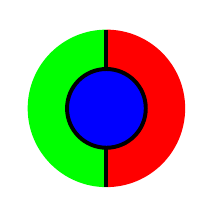
\begin{tikzpicture}
            \fill[blue] (0,0) circle(0.5);
    
            \fill[red]
            (0,-0.5)           % Start at bottom inner point
            arc(-90:90:0.5)     % Inner arc: radius=0.5 from -90° to 90° (bottom to top on the right side)
            -- (0,1)            % Line from top inner (0,0.5) to top outer (0,1)
            arc(90:-90:1)       % Outer arc: radius=1 from 90° to -90° (top to bottom on the right side)
            -- cycle;           

            \begin{scope}[rotate=180]
            \fill[green]
            (0,-0.5)
            arc(-90:90:0.5)
            -- (0,1)
            arc(90:-90:1)
            -- cycle;
            \end{scope}
            
            % Decision boundary
            \draw[line width=0.5mm] (0, 0.5) -- (0, 1);
            \draw[line width=0.5mm] (0, -0.5) -- (0, -1);
            \draw[line width=0.5mm] (0,0) circle (0.5);
        \end{tikzpicture}
        \caption{All classes shown}
        \label{fig:binarization:all}
    \end{subfigure}
    \begin{subfigure}[b]{0.3\textwidth}
        \centering
        
\begin{tikzpicture}
            \fill[red]
            (0,-0.5)           % Start at bottom inner point
            arc(-90:90:0.5)     % Inner arc: radius=0.5 from -90° to 90° (bottom to top on the right side)
            -- (0,1)            % Line from top inner (0,0.5) to top outer (0,1)
            arc(90:-90:1)       % Outer arc: radius=1 from 90° to -90° (top to bottom on the right side)
            -- cycle;           

            \begin{scope}[rotate=180]
            \fill[green]
            (0,-0.5)
            arc(-90:90:0.5)
            -- (0,1)
            arc(90:-90:1)
            -- cycle;
            \end{scope}
            
            % Decision boundary
            \draw[line width=0.5mm] (0, 0.5) -- (0, 1);
            \draw[line width=0.5mm] (0, -0.5) -- (0, -1);
        \end{tikzpicture}
        \caption{Red and green classes}
        \label{fig:binarization:rg}
    \end{subfigure}
    \begin{subfigure}[b]{0.3\textwidth}
        \centering
        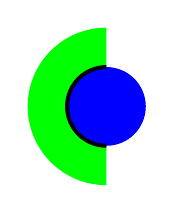
\begin{tikzpicture}
            \fill[blue] (0,0) circle(0.5);
    
            \begin{scope}[rotate=180]
            \fill[green]
            (0,-0.5)
            arc(-90:90:0.5)
            -- (0,1)
            arc(90:-90:1)
            -- cycle;
            \end{scope}
            
            % Decision boundary
            \draw[line width=0.5mm] (0,0.5) arc (90:270:0.5);
        \end{tikzpicture}
        \caption{Green and blue classes}
        \label{fig:binarization:gb}
    \end{subfigure}
    \caption{A 2D example that demonstrates the loss of topological information when binarizing a multiclass dataset. Red, green and blue denote different classes, the black line is the decision boundary.}
    \label{fig:binarization}
\end{figure}

To avoid this information loss, we propose a generalization of
the Labeled Vietoris-Rips complex to multiclass classification.
For a labeled discrete sample \(\{(z_1, c_1), \dots, (z_n, c_n)\}\),
where \(z \in \R^d\) is a data point and \(c \in \{1, \dots, n\}\) is its class,
we define a bipartite graph \(G_\theta\) by
adding an endge between \(z_i\) and \(z_j\) iff \(c_i \neq c_j\)
and \(\norm{z_i - z_j} \leq \theta\).
\todo{Say how this is a no-op compared to LVR}
\todo{Say we don't generalize LC}

To combat issues shown in \ref{sec:2d-issues}, we propose \emph{circumcircle filtering} (CC).
CC removes an edge between points \(A\) and \(B\) from the simplicial complex
if exists a point \(C\) such that \(|AB|^2 > (|AC|^2 + |BC|^2) \theta\),
where \(\theta \in [0, 2]\) is a parameter.
Intuitively, this approach aims to make a simplicial complex more similar
to the Alpha complex \todo{cite} by removing some (but not all) non-Delaunay edges.
\todo{Explain this better}

Alternatively, we propose usage of the \emph{Dowker complex} to combat the same issues.
However, computing it requires \(\mathcal{O}(n^3 \cdot d)\) runtime and \(\mathcal{O}(n^3)\)
memory for \(n\) points in \(\R^d\), which is prohibitively expensive
for the MNIST and FashionMNIST datasets.
Additionally, the Dowker complex is not applicable in the multiclass setting.
Nonetheless, we demonstrate its effectiveness on 2D data in \ref{sec:2d-issues}.
\todo{Confirm complexity}